\documentclass[10pt,a4paper]{report}
\usepackage[utf8]{inputenc}
\usepackage[spanish]{babel}
\usepackage{amsmath}
\usepackage{amsfonts}
\usepackage{amssymb}
\usepackage{wallpaper}
\usepackage{cite}
\usepackage{graphicx}
\usepackage{wrapfig}
\usepackage{multirow}
\usepackage{lmodern}
\author{José Márquez de Prado}
\title{Mejores coches japoneses}

\begin{document}
\begin{titlepage}
\begin{huge}
\textbf{Los mejores coches de Japón.}
\end{huge}
\begin{wrapfigure}{l}{10mm}
  \begin{center}
    
\includegraphics[scale=.45]{Solnaciente.jpg}
  \end{center}
\end{wrapfigure}
\end{titlepage}
Japón, tierra del sol naciente, siempre ha destacado por tener vehículos muy rápidos, muy competitivos y con buenos motores bastante fiables, que han conseguido competir con los automóviles de alta gama de Europa o EEUU y revolucionar la fórmula del despazamiento $\Delta_x = x_f - x_i$ para siempre.

Si hay que destacar una época concreta en el mundo de los automóviles japoneses esa es la era de los 90; y, si hay que elegir una marca, cosa que sería muy difícil y que iría al gusto de cada uno, yo me quedaría con Honda, marca de la cual vamos a comentar los modelos más representativos.

De igual modo, antes veremos resumidamente los modelos japoneses que más han destacado en la historia:

\begin{table}[htbp]
\begin{center}
\begin{tabular}{|l|l|l|l|l|}
\hline
Marca & Modelo & Motor & Potencia & Fabricación \\
\hline \hline
Honda & Civic & B18 & 169hp & 1992 \\ \hline
Honda & NSX & C30A & 280hp & 1990 \\ \hline
Honda & S2000 & F22C1 & 250hp & 2000 \\ \hline
Mazda & MX5 & NC & 160hp & 1990 \\ \hline
Mazda & RX8 & Wankel & 231hp & 2002 \\ \hline
Mitsubishi & 3000GT & 5G72 & 296hp & 1990 \\ \hline
Mitsubishi & Lancer EVO & B18 & 169hp & 1992 \\ \hline
Nissan & Silvia S15 & R-I4 & 250hp & 1999 \\ \hline
Nissan & Skyline R34 & RB26DETT & 280hp & 1993 \\ \hline
Nissan & 370Z & VQ37VHR & 333hp & 2009 \\ \hline
Toyota & Corolla AE86 & 4A-C & 87hp & 1985 \\ \hline
Toyota & Supra & 2JZ-GE & 326hp & 1993 \\ \hline
\end{tabular}
\label{tabla:sencilla}
\end{center}
\end{table}
\subsection{Honda Civic}
El Honda Civic es un automóvil del segmento C fabricado por Honda Motor Co. Tras pasar por varios cambios generacionales, es un vehículo que ha crecido en tamaño, colocándose entre el Honda Fit y el Honda Accord.
Todos los modelos, hasta el momento, poseen un motor delantero transversal de 4 cilindros, tracción delantera y varias carrocerías:
\begin{enumerate}
\item Sedan.
\item Coupé.
\item Hatchback.
\item Aerodeck.
\end{enumerate}

El vehículo fue introducido en julio de 1972 como un modelo de 2 puertas, seguido de un hatchback de 3 puertas, ambos con motor transversal de 1169cc y tracción delantera.
Se trata de un coche que ganó su reputación gracias a su eficiencia y su bajo consumo, y por ser seguro y respetuoso con el medio ambiente. Las versiones posteriores se han dado a conocer por el rendimiento y la deportividad, especialmente la versión Type-R.
\\
\begin{wrapfigure}{l}{80mm}
  \begin{center}
    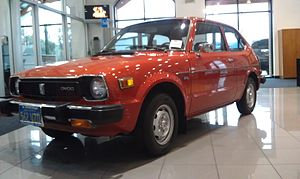
\includegraphics[scale=.45]{civic1.jpg}
  \end{center}
  \caption{Primera Generación}
\end{wrapfigure}
La primera generación de Honda Civic recibió durante 3 años consecutivos, desde 1972 hasta 1974, el premio \textbf{Coche del Año en Japón}, y quedando tercero en la elección de \textbf{Coche del Año en Europa}, mejor resultado obtenido nunca por un coche japonés.
\\ \\
La segunda generación de Honda Civic fue lanzada en 1979. Era más grande, tenía una forma más angular y mayor potencia que su predecesor.
Este coche usaba, al igual que la primera generación, un motor de diseño CVCC que destacaba por sus bajas emisiones y su bajo consumo, añadiendo uan tercera válvula por cilindro y pasando de 8 a 12 válvulas.
Como transmisión había 4 variedades posibles: una versión manual de 4 velocidades, una versión manual de 5 velocidades, y una de 2 velocidades semiautomática llamada \textit{Hondamatic}.
\\

La tercera generación fue presentada en 1983. Paralelamente se lanzó un coupé 2+2 asientos llamado CR-X, que destacaba por su tamaño compacto y peso ligero.\\
El concepto para la tercera generación del Civic fue "espacio máximo para las personas, espacio mínimo para los mecanismos". Basándose en este concepto, Honda desarrolló variantes hatchback de tres y cinco puertas y un sedán de cuatro puertas. El Civic ganó el premio al "Coche del Año 1984 en Japón". En 1984, el Civic obtuvo la primera posición en las pruebas de consumo de combustible realizadas por la agencia de protección del medio ambiente de los Estados Unidos por segundo año consecutivo. En Europa, ganó el premio al "Mejor Diseño".\\
El vehículo venía equipado con suspensiones delanteras con barra de torsión independientes y suspensiones traseras semi-independientes de barras de torsión con espirales helicoidales, techo solar, discos de freno en el tren delantero de 241mm ventilados con pinzas de pistón simple y frenos de tambor en el eje trasero. Las motorizaciones equipadas en este modelo fueron los motores denominados D15A1, D15A2, D15A3 y D15A4.
\\

En 1987, el Civic fue rediseñado con mayores dimensiones y una línea de capó más baja.
De esta generación destaca el modelo "Civic SiR" presentado en 1989, iba equipado con un motor con doble árbol de levas en cabeza y la revolucionaria tecnología de distribución de válvulas variable llamada VTEC por Honda. Este modelo ha ganado numerosos premios, entre ellos el "Golden Steering Wheel Award" de Alemania. También quedó en primera posición en la encuesta sobre calidad realizada en Francia en 1989.
\\
Los modelos más notables que se incluyeron en el mercado, fueron el Civic SiR japonés o el Civic VTi Europeo (ambos con el nuevo motor B16A DOHC VTEC), el 1.6i-16 (DOHC D16A9) en el Reino Unido/Europa.
\\
\begin{wrapfigure}{l}{70mm}
  \begin{center}
    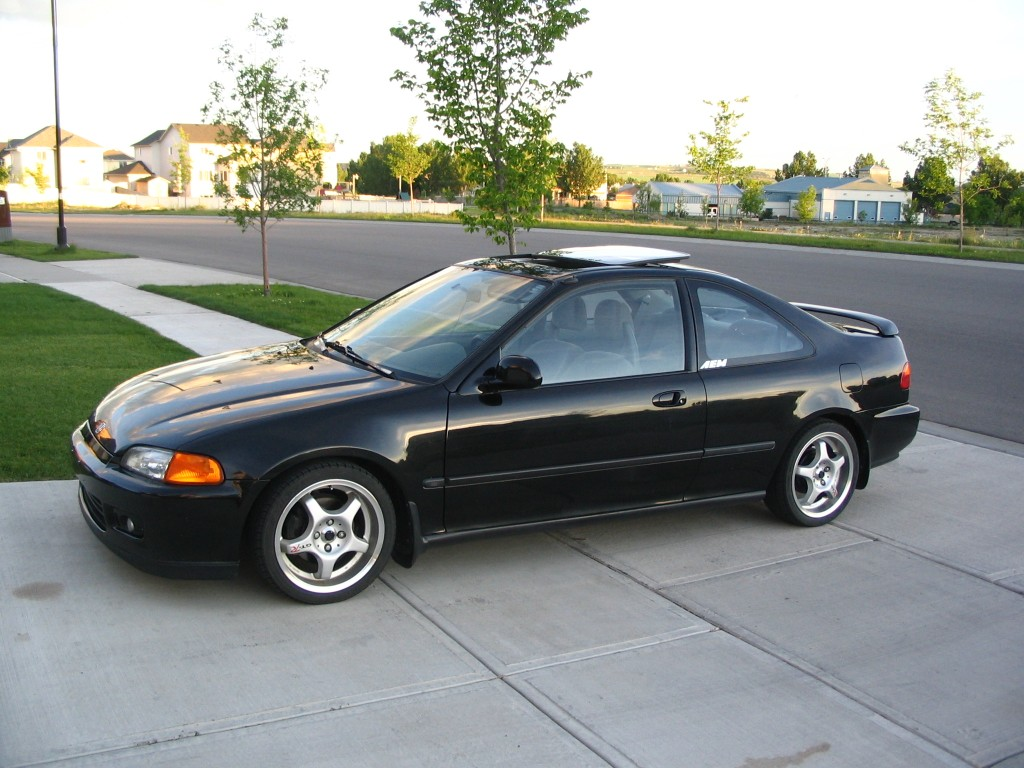
\includegraphics[scale=0.20]{ej1a.jpg}
  \end{center}
  \caption{Civic EJ1}
\end{wrapfigure}
La quinta generación, lanzada en 1991, es una de las preferidas por los consumidores, destacando su futurista línea aerodinámica, con una gran flexibilidad de espacio interior.
Esta generación es muy usada en las competiciones de Drag de 1/4 de milla, donde los motores B16 y B18 VTEC de 160 y 169hp destacan por su potencia y aceleración.
\begin{equation}
V_m = \frac{Espacio\ recorrido}{Tiempo\ empleado}
\end{equation}
Este modelo en concreto, junto a las preparaciones que le han hecho sus distintos usuarios, han hecho locuras con esta fórmula, yendo las motorizaciones de los 90hp que trae el modelo más basico de Honda Civic 5ª generación, a más de 1000hp que tienen las preparaciones más locas del mundo del Drag.
\\

La sexta generación del Civic montaba los motores D16Y8 SOHC VTEC de 125 CV en el EJ8 y D16Y7 en el EJ6 (sin VTEC) de 105 CV ambas versiones Coupe. En las versiones de 3 puertas encontramos los motores D15Z6 SOHC VTEC-E que rinde 115 CV (EK3), D14A3/A4/Z2 que rinde 90 CV sin VTEC (EJ9). También se produjo el modelo deportivo VTI con un motor de B16A2 DOHC VTEC que entrega una potencia de 160 cv, y la versión Type-R de 185 CV que montaba el motor B16B era denominado EK9 y estaba solo disponible en el mercado Japonés. Recibió un ligero reestyling en el año 1998.
\\
También se creó una versión 5 puertas denominado MA/MB (Sedan) y MC (Aerodeck) de venta solo en Europa.

\begin{wrapfigure}{r}{50mm}
    \includegraphics[scale=0.50]{fn2.jpg}
  \caption{Civic Type-R}
\end{wrapfigure}
Con un diseño altamente revolucionario, alejado de lo que ya se conocía del Honda Civic, esta octava generación presentó un diseño avanzadamente aerodinámico, que poco conservaba de sus antecesores. Con estos argumentos, Honda decidió darle a esta octava generación del Civic, el nombre comercial de Honda New Civic, representando la renovación total del coche insignia de la marca japonesa.//

El Civic de octava generación consta de cuatro motorizaciones gasolina en opa: un 1.4 litros de 83 CV hasta 2008 y de 100 CV en el modelo 2009 en adelante, un 1.8 litros de 140 CV y un 2.0 litros de 201 CV. Los cuatro son atmosféricos.

\newpage
\subsection{Honda NSX}
\begin{wrapfigure}{r}{60mm}
    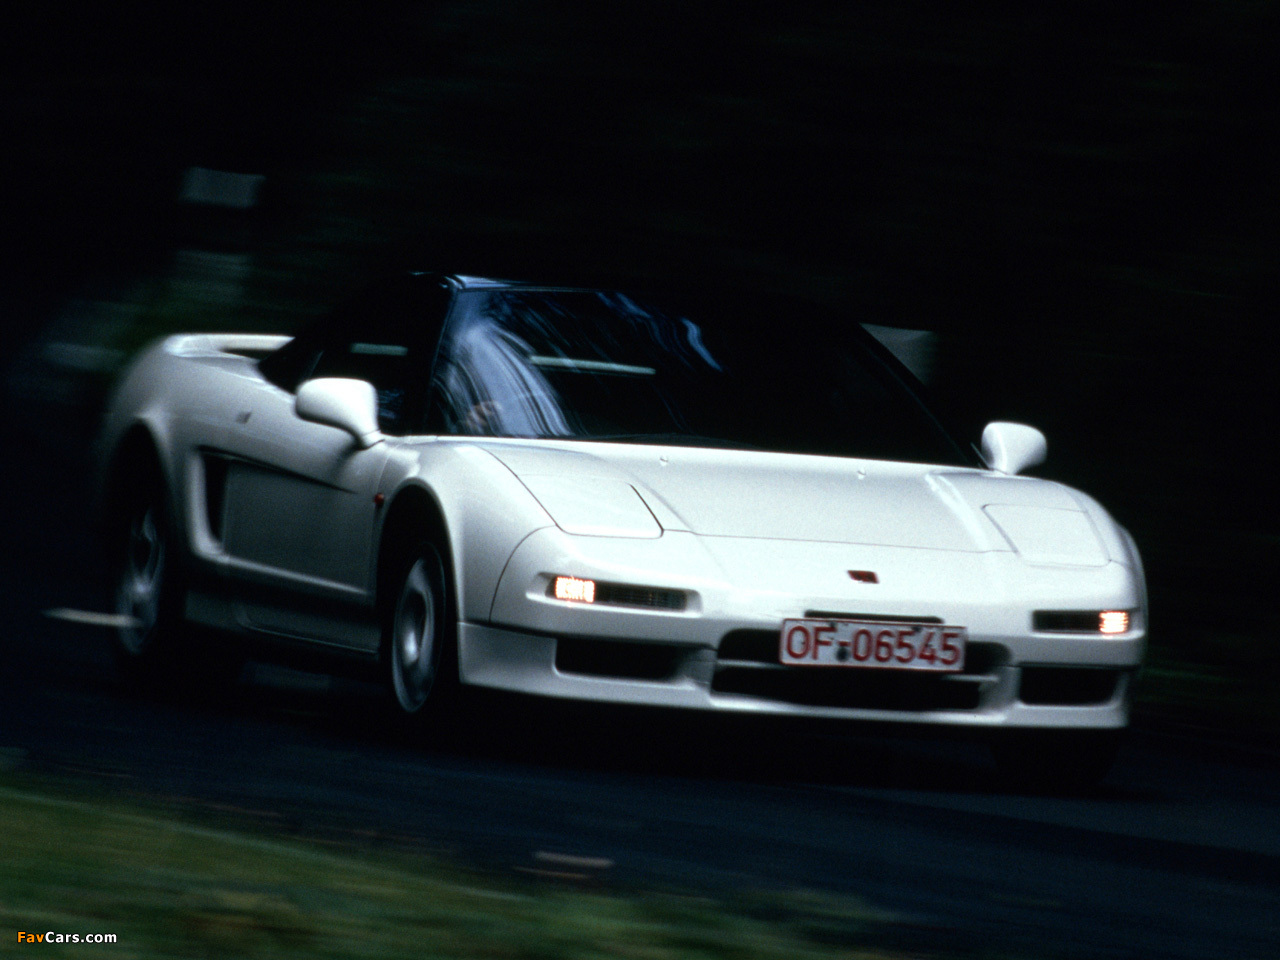
\includegraphics[scale=0.90]{na1.jpg}
  \caption{Honda NSX NA1}
\end{wrapfigure}
Fabricado por Honda, y por su filial para coches de gama alta, Acura, el NSX es uno de los mejores coches de la historia, conocido como \textit{el antiferrari}, debido a que podía competir contra éstos y hacer mejores tiempos.\\
Se trata de un automóvil de 2 plazas, motor central y carrocería coupé y targa, fabricado entre 1990 y 2005, y refabricado en 2012.
Estuvo inspirado en el avión  F-16 Fighting Falcon y el piloto de Fórmula 1 Ayrton Senna fue el encargado de probar esta máquina antes de sacarla a producción en el circuito de Nürburgring.
\\

\begin{table}[htbp]
\begin{center}
\begin{tabular}{|l|l|}
\hline
\textbf{NSX NA1} \\
\hline \hline
Motor & V6 DOHC VTEC. Culata y bloque motor de aleación \\ \hline
Desplazamiento & 2977cc (90x78 mm) \\ \hline
Potencia & 270cv (266 Hp)(201kW) a 7100 rpm \\ \hline
Par maximo & 284 Nm a 5400 rpm \\ \hline
Velocidad maxima & 270 km/h \\ \hline
Aceleración 0-100 km/h & 5.9s \\ \hline
Consumo de combustible & Ciudad: 13,8L/100 km \\ \hline
Precio de compra & NSX (1992) 11.500.000 pta \\ \hline
\end{tabular}
\label{tabla:sencilla}
\end{center}
\end{table}

Al modelo NA1 siguió el modelo NA2, con un diseño muy parecido que difería en los pilotos traseros, de un diseño más moderno y en los faros delanteros, que dejaron de ser escamoteables.
En cuanto al motor, era muy parecido pero el NA2 ofrecía algo más de potencia, pasando de ser de un 3.0 a un 3.2 y cambiando la potencia de 270hp a 280hp.
\\

Tras 10 años sin comercialización de ninguno de los 2 modelos de NSX, Honda anunció un nuevo modelo en 2012, siendo presentado en el Salón de Detroit de 2015. Este nuevo vehículo se comercializaría con un precio de 143.500 euros el modelo básico, y 189.200 euros el modelo con todos los extras.\\
En cuanto a motor, contará con un motor V6 3.5 con doble turbo, que formará parte del sistema \textbf{SH-AWD (Sport Hybrid - All Wheel Drive}), incluyendo doble embrague y 9 marchas, y un motor eléctrico situado entre el motor de propulsión y la transmisión, junto a otros 2 motores eléctricos frontales.\\

El motor V6 de 3.5 litros sobrealimentado producirá 506 CV y 550 Nm de par. Junto a él, un pequeño motor eléctrico proporcionará otros 50 CV y unos respetables 135 Nm de par instantáneos. Este motor será de apoyo y estará colocado tras la transmisión automática de nueve velocidades. 
En la parte delantera los protagonistas serán dos motores eléctricos con una potencia de 40 CV y 72 Nm de par cada uno. Estos se encargarán de mover las ruedas delanteras y de proporcionar la tracción integral. \\
\begin{wrapfigure}{l}{90mm}
  \begin{center}
    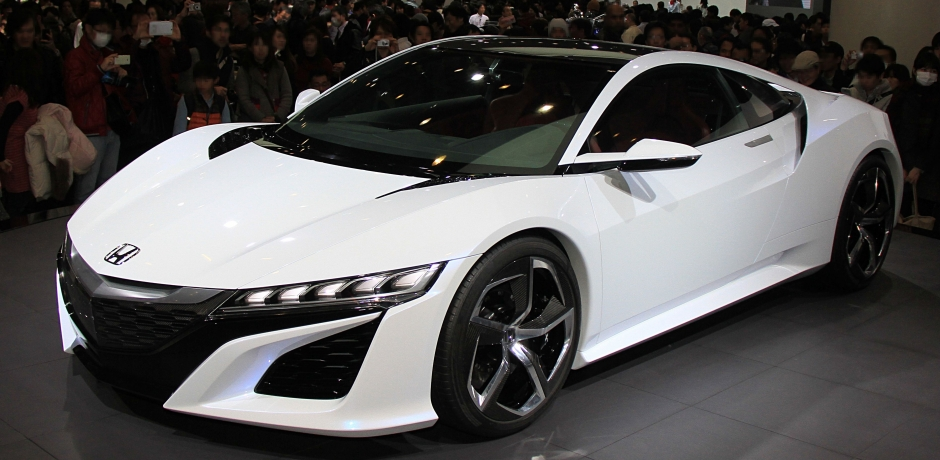
\includegraphics[scale=.25]{nsx2015.jpg}
  \end{center}
    \caption{Honda NSX 2015}
\end{wrapfigure}
Así pues, la potencia conjunta de todos estos motores eléctricos y de combustión ya tiene una cifra oficial: 580 CV y 644 Nm de par. Con semejante torrente de potencia y gracias al par instantáneo de los motores eléctricos, cuando todo funcione a máximo rendimiento se podrá acelerar de 0 a 100 en apenas 3 segundos, mientras que la velocidad máxima será de 307 km/h. Todo para un coche que tan sólo pesa 1.725 kg
\\

\subsection{Honda S2000}

Terminamos este artículo con el Honda S2000, un coche que en su día sustituyó al Honda CRX del Sol, variante del CRX que, a su vez, fue una variante del Honda Civic.\\
El Honda S2000 es un coche descapotable de 2 plazas creado para celebrar el 50 aniversario de la marca japonesa, y fue la continuación de los roadsters S500, S600 y S800. \\
El vehículo posee un diferencial de deslizamiento limitado \textbf{Torsen} acoplado a una transmisión manual de 6 velocidades.
\\

De este modelo existen 2 versiones, denominadas AP1 y AP2. Ambas son prácticamente idénticas y las únicas diferencias se notan en la forma de los faros y pilotos traseros, y en la forma de los paragolpes.
\\

El S2000 estaba equipado con un motor de 4 cilindros en línea DOHC-VTEC con denominación interna F20C de 2.0 L (1997 cc) que producía 220 hp a 8.300 rpm y un par motor de 208 Nm a 7.500 rpm en las unidades destinadas al mercado norteamericano. Las unidades destinadas a Europa tenían 240 hp (177 kW) y los modelos destinados a Japón 250 hp a 8.600 rpm debido a pequeñas diferencias en la relación de compresión del motor.
\\

Honda introdujo una variante del motor F20C en el mercado norteamericano en 2004. Designado F22C1, la carrera del pistón fue incrementada haciendo que la cilindrada del motor pasara a 2.2 L. La zona roja se redujo de 9.000 a 8.000 rpm con el corte de inyección a 8.200 rpm, debido a la mayor carrera del pistón.\\ El par máximo se incrementó hasta 220 Nm a 6.200 rpm, y el F22C1 fue puesto a punto para tener mayor par a bajas revoluciones que el F20C, aunque la potencia máxima era la misma. Inicialmente, el F22C1 solo estaba destinado al mercado norteamericano, pero fue introducido en Japón en 2006 con 242 hp. En el resto de mercados continua la versión de 2.0 L.
\begin{center}
    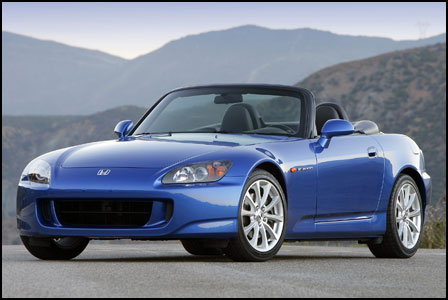
\includegraphics[scale=.65]{s2000.jpg}
\end{center}
Debido en parte a la naturaleza de su motor de altas revoluciones (corte a 9.000 rpm en el 2,0L y 8.200 rpm en el 2,2L), el S2000 logra la mayor potencia específica de cualquier motor de pistones atmosférico producido en serie en el mundo, con 125 hp en el F20C japonés.
\\

Al introducir el F22C1, Honda cambio también los desarrollos de la transmisión acortando las 4 primeras marchas y alargando las otras 2. Otra inclusión fue una válvula de liberación del embrague que incrementaba la longevidad de la transmisión.\\

\bibliographystyle{acm}
\bibliography{biblio}

\end{document}